\documentclass{article}

\def\ParSkip{} 
% Packages
\usepackage{amssymb,amsmath,amsthm,bbm}
\usepackage{verbatim,float,url,dsfont}
\usepackage{graphicx,subfigure,psfrag}
\usepackage{algorithm,algorithmic}
\usepackage{mathtools,enumitem}
\usepackage{multirow}
\usepackage{ragged2e}
\usepackage{xr-hyper}
\usepackage{array}

\usepackage[colorlinks=true,citecolor=blue,urlcolor=blue,linkcolor=blue]{hyperref}
\usepackage[margin=1in]{geometry}
\usepackage[round]{natbib}

\usepackage[utf8]{inputenc} % allow utf-8 input
\usepackage[T1]{fontenc}    % use 8-bit T1 fonts
\usepackage{booktabs}       % professional-quality tables
\usepackage{nicefrac}         % compact symbols for 1/2, etc.
\usepackage{microtype}      % microtypography

\ifdefined\TimesFont 
\usepackage{times} % use times font
\fi

\ifdefined\ParSkip 
\usepackage{parskip} % use par skip
\fi

% Theorems and such
\newtheorem{theorem}{Theorem}
\newtheorem{lemma}{Lemma}
\newtheorem{corollary}{Corollary}
\newtheorem{proposition}{Proposition}
\theoremstyle{definition}
\newtheorem{remark}{Remark}
\newtheorem{definition}{Definition}

% Assumption
\newtheorem*{assumption*}{\assumptionnumber}
\providecommand{\assumptionnumber}{}
\makeatletter
\newenvironment{assumption}[2]{
  \renewcommand{\assumptionnumber}{Assumption #1#2}
  \begin{assumption*}
  \protected@edef\@currentlabel{#1#2}}
{\end{assumption*}}
\makeatother

% Widebar
\makeatletter
\newcommand*\rel@kern[1]{\kern#1\dimexpr\macc@kerna}
\newcommand*\widebar[1]{%
  \begingroup
  \def\mathaccent##1##2{%
    \rel@kern{0.8}%
    \overline{\rel@kern{-0.8}\macc@nucleus\rel@kern{0.2}}%
    \rel@kern{-0.2}%
  }%
  \macc@depth\@ne
  \let\math@bgroup\@empty \let\math@egroup\macc@set@skewchar
  \mathsurround\z@ \frozen@everymath{\mathgroup\macc@group\relax}%
  \macc@set@skewchar\relax
  \let\mathaccentV\macc@nested@a
  \macc@nested@a\relax111{#1}%
  \endgroup
}
\makeatother

% Min and max
\newcommand{\argmin}{\mathop{\mathrm{argmin}}}
\newcommand{\argmax}{\mathop{\mathrm{argmax}}}
\newcommand{\minimize}{\mathop{\mathrm{minimize}}}
\newcommand{\maximize}{\mathop{\mathrm{maximize}}}
\newcommand{\st}{\mathop{\mathrm{subject\,\,to}}}

% Shortcuts
\def\R{\mathbb{R}}
\def\C{\mathbb{C}}
\def\Z{\mathbb{Z}}
\def\N{\mathbb{N}}
\def\E{\mathbb{E}}
\def\P{\mathbb{P}}
\def\T{\mathsf{T}}
\def\Cov{\mathrm{Cov}}
\def\Var{\mathrm{Var}}
\def\indep{\perp\!\!\!\perp}
\def\th{^{\text{th}}}
\def\tr{\mathrm{tr}}
\def\df{\mathrm{df}}
\def\dim{\mathrm{dim}}
\def\col{\mathrm{col}}
\def\row{\mathrm{row}}
\def\nul{\mathrm{null}}
\def\rank{\mathrm{rank}}
\def\nuli{\mathrm{nullity}}
\def\spa{\mathrm{span}}
\def\sign{\mathrm{sign}}
\def\supp{\mathrm{supp}}
\def\diag{\mathrm{diag}}
\def\aff{\mathrm{aff}}
\def\conv{\mathrm{conv}}
\def\dom{\mathrm{dom}}
\def\hy{\hat{y}}
\def\hf{\hat{f}}
\def\hmu{\hat{\mu}}
\def\halpha{\hat{\alpha}}
\def\hbeta{\hat{\beta}}
\def\htheta{\hat{\theta}}
\def\cA{\mathcal{A}}
\def\cB{\mathcal{B}}
\def\cD{\mathcal{D}}
\def\cE{\mathcal{E}}
\def\cF{\mathcal{F}}
\def\cG{\mathcal{G}}
\def\cK{\mathcal{K}}
\def\cH{\mathcal{H}}
\def\cI{\mathcal{I}}
\def\cL{\mathcal{L}}
\def\cM{\mathcal{M}}
\def\cN{\mathcal{N}}
\def\cP{\mathcal{P}}
\def\cS{\mathcal{S}}
\def\cT{\mathcal{T}}
\def\cW{\mathcal{W}}
\def\cX{\mathcal{X}}
\def\cY{\mathcal{Y}}
\def\cZ{\mathcal{Z}}


\title{High-Dimensional Regression: Ridge \\ \smallskip
\large Advanced Topics in Statistical Learning, Spring 2023 \\ \smallskip
Ryan Tibshirani}
\date{}

\begin{document}
\maketitle
\RaggedRight
\vspace{-50pt}

Note: we're following the context, problem setup, notation, etc. from the last
lecture on high-dimensional regression.

\section{Ridge basics}

We'll jump right into some basic properties of \emph{ridge regression}, which
recall, for a predictor matrix $X \in \R^{n \times d}$ and response vector $Y
\in \R^n$, is defined by
\begin{equation}
\label{eq:ridge}
\minimize_\beta \; \|Y - X\beta\|_2^2 + \lambda \|\beta\|_2^2, 
\end{equation}
for a tuning parameter $\lambda \geq 0$. Unlike the lasso and best subset
selection (which replace the $\|\beta\|_2^2$ penalty above with $\|\beta\|_1$
and $\|\beta\|_0$, respectively), recall, the solution in the ridge problem
\eqref{eq:ridge} is generically dense: it has all nonzero components, for any
$\lambda > 0$.  

Yes, above we said \emph{the} solution in \eqref{eq:ridge}, and that was 
intentional. For any $\lambda > 0$, the criterion in the problem
\eqref{eq:ridge} is strictly convex, due to the $\lambda \|\beta\|_2^2$ term. It
therefore always has a unique solution (regardless of $X$). There is not much
else to say, except to emphasize the contrast here to the lasso problem, which,
recall, does not always admit a lasso solution, though we were able to do some
basic analysis to show that it has a unique solution whenever $X$ has columns in
general position.      

More than just being unique, the solution in \eqref{eq:ridge} has an explicit
form,
\begin{equation}
\label{eq:ridge_sol}
\hbeta = (X^\T X + \lambda I)^{-1} X^\T Y,
\end{equation}
for $\lambda > 0$. As another way to see the uniqueness claim, note that $X^\T X
+ \lambda I$ is always invertible whenever $\lambda > 0$, since its smallest
eigenvalue is at least $\lambda$. 

Now, there are many ``facets'' of the ridge regression estimator, by which we
mean, many perspectives from which to view it. We'll walk through a number of
these now (there are many others we don't cover!), before moving to the tools
needed to analyze the risk of ridge regression.   

\subsection{Principal components view}

A standard way to view the ridge regression estimator is through the lens of how
it acts in principal components space. Let $X = U \Sigma V^\T$ be a singular
value decomposition of $X$. Then we can write the vector of ridge fitted values
as: 
\begin{align*}
X\hbeta &= X (X^\T X + \lambda I)^{-1} X^\T Y \\
&= U \Sigma^2 (\Sigma^2 + \lambda I)^{-1} U^\T Y \\ 
&= \sum_{j=1}^n \frac{\sigma_j^2}{\sigma_j^2+\lambda} u_j u_j^\T Y,  
\end{align*}
where $u_j$ denotes the $j\th$ column of $U$, and $\sigma_j$ the $j\th$ diagonal 
element of $\Sigma$. Note that the least squares projection of $Y$ on $X$
(always well-defined, even if $d > n$) is
\[
U U^\T Y = \sum_{j=1}^n u_j u_j^\T Y.
\]
Comparing the second-to-last display to the last one, we can see that ridge 
(compared to least squares) performs shrinkage, but not uniformly so in all 
directions---it shrinks more along the principal component directions $u_j$ that
correspond to low variance (small $\sigma_j$), and less along the directions
$u_j$ that correspond to high variance (large $\sigma_j$).    

\subsection{Bayesian view}

Another standard way to view ridge regression is as a Bayes estimator in a 
normal-normal model for the likelihood and prior. That is, for fixed $X$,
consider the model 
\begin{equation}
\label{eq:normal_bayes}
\begin{aligned}
\beta &\sim N(0, \frac{1}{\lambda} I), \\
Y | \beta &\sim N(X\beta, I).
\end{aligned}
\end{equation}
Then, following standard calculations in Bayesian inference, where we often use
$p(\cdot)$ to denote the density of its argument, it holds that
\[
p(\beta | Y) \propto p(Y | \beta) \, p(\beta),
\]
where $\propto$ means ``proportional to'' and ignores terms not depending on
$\beta$. Again by standard calculations, the right-hand side above can be
identified as proportional to a Gaussian density. Therefore (because it is
Gaussian), its mean is equal to its mode, and the Bayes estimator is the maximum 
a posteriori (MAP) estimator:
\begin{align}
\nonumber
\E[\beta | Y] &= \argmax_\beta \; p(Y | \beta) \, p(\beta) \\
&= \argmin_\beta \; -\log p(Y | \beta) - \log p(\beta) \\
\label{eq:ridge_bayes}
&= \argmin_\beta \; \frac{1}{2} \|Y - X\beta\|_2^2 + \frac{1}{2\lambda}
  \|\beta\|_2^2,
\end{align}
that is, the Bayes estimator in this model is simply the ridge estimator. 

We note that the lasso can also be written as a MAP estimator in a Bayesian 
model, where the prior in \eqref{eq:normal_bayes} is now Laplace rather than  
Gaussian. However, the MAP estimator is \emph{not} the Bayes estimator
(posterior expectation) in this particular model: the posterior is no longer
Gaussian and no longer has the property of symmetry around its mode that would
imply its mode and its mean are the same.   

\subsection{Kernel view}

Another interesting view stems from what is called the push-through matrix
identity:
\begin{equation}
\label{eq:push_through}
(aI + UV)^{-1} U = U (aI + VU)^{-1}.
\end{equation}
for $a,U,V$ such that the products are well-defined and the inverses exist. We
can obtain this from
\[
U (aI + UV) = (aI + UV) U,
\]
followed by multiplication by $(aI + UV)^{-1}$ on the left and the right. 
Applying the identity \eqref{eq:push_through} to \eqref{eq:ridge_sol} with
$a=\lambda$, $U=X^\T$, and $V=X$, we obtain an alternative form for the ridge
solution:  
\begin{equation}
\label{eq:ridge_kernel}
\hbeta = X^\T (XX^\T + \lambda I)^{-1} Y.
\end{equation}
This is often referred to as the kernel form of the ridge estimator. From
\eqref{eq:ridge_kernel}, we can see that the ridge fit can be expressed as
\[
X\hbeta = XX^\T (XX^\T + \lambda I)^{-1} Y.
\]
What does this remind you of? This is precisely $K(K + \lambda I)^{-1} Y$ where
$K = XX^\T$, which, recall, is the fit from RKHS regression with a linear kernel 
$k(x,z) = x^\T z$. Therefore we can think of RKHS regression as generalizing
ridge regression, by replacing the standard linear inner product with a general
kernel. (Indeed, RKHS regression is often called kernel ridge regression.)

\subsection{Noise features view}

\def\asto{\overset{\mathrm{as}}{\to}}

The last view we cover is likely the least well-known, but it is still very 
interesting. This is due to \citet{kobak2020optimal}. Suppose that we append to
the columns of our feature matrix $X \in \R^{n \times d}$ a large number of
``noise'' features $Z \in \R^{n \times D}$ where $D$ is very large and each
$Z_{ij}$ is stochastic with mean zero and variance $\tau^2$, independent of
$Y$. Denote such an augmented feature matrix by
\[
\tilde X = [X; Z] \in \R^{n \times (d+D)},
\]
and consider performing least squares regression---with no explicit ridge
regularization---of $Y$ on \smash{$\tilde{X}$}. As we are considering the large
$D$ limit, we will inevitably have $d+D > n$ at some point, so we'll need to
amend the least squares estimator because it is nonunique and has the
pathologies we already discussed. To do so, we'll take the \emph{minimum 
  $\ell_2$ norm least squares solution}, 
\begin{equation}
\label{eq:ls_noise}
\tilde\beta = (\tilde X^\T \tilde X)^+ \tilde X^\T Y.
\end{equation}
We'll also simply call this the min-norm solution (especially when it is
unambiguous from the context that the norm we're talking about is
$\ell_2$). We'll spend a lot more time discussing min-norm least squares when we
talk about overparametrization theory, in the next lecture.  

Now we rewrite \eqref{eq:ls_noise} in kernel form. By even simpler arguments
than those in the previous subsection---just using the fact tha the generalized 
inverse and transpose operations commute in general, $(A^+)^\T = (A^\T)^+$---we 
can rewrite the min-norm solution (assuming that $d+D > n$ and \smash{$\tilde
  X$} has full row rank) as  
\begin{align*}
\tilde\beta &= \tilde X^\T (\tilde X \tilde X^\T)^{-1} Y \\
&= [X; Z]^\T (XX^\T + ZZ^\T)^{-1} Y \\
&= [X; \tau \tilde Z]^\T (XX^\T + \tau^2 \tilde Z \tilde Z^\T)^{-1} Y,  
\end{align*}
where in the last line we have rescaled the noise features so that each
\smash{$\tilde Z_{ij} = \tau^{-1} Z_{ij}$} has zero mean and unit variance. If 
we take \smash{$\tau = \sqrt{\lambda/D}$}, then by the law of large numbers, 
\[
\frac{\lambda}{D} \tilde Z \tilde Z^\T \asto \lambda I, \quad \text{as $D \to
  \infty$}. 
\]
Therefore if we let \smash{$\tilde \beta_{[d]}$} denote the first $d$ components
of the min-norm least squares solution in \eqref{eq:ls_noise} (which has total
dimension $d+D$), then   
\[
\tilde \beta_{[d]} \asto X^\T (XX^\T + \lambda I)^{-1} Y, \quad \text{as $D \to 
  \infty$},
\]
the limit here being the ridge solution from regressing $Y$ on $X$ with tuning
parameter $\lambda$. Similarly, for any fixed $\tilde x = (x, z) \in \R^{d+D}$,  
\[
\tilde x^\T \tilde \beta \asto x^\T X^\T (XX^\T + \lambda I)^{-1} Y, \quad
\text{as $D \to \infty$},
\]
the limit here being the ridge prediction from regressing $Y$ on $X$ with tuning
parameter $\lambda$. In other words, min-norm least squares on an augmented
design where we augment the given features with noise features---whose variance
vanishes appropriately as the number of them grows---reproduces ridge
regression! 

\section{Random matrix theory}

In this section, we will introduce some basic results in random matrix theory
(RMT), which will serve as the backbone that we will use to analyze the risk of
ridge regression in the rest of the lecture. As an editorial remark, you'll
often hear ``random matrix theory'' to describe two generally related but
different flavors of results: asymptotic and non-asymptotic. Below we will be
talking about asymptotic RMT. And as per our usual comment, there is a lot to 
learn about random matrix theory and we're only really covering the tip of the
iceberg; to learn more, well beyond what we cover here, see, e.g.,
\citet{tulino2004random, bai2010spectral}, which are definitive references for
the type of asymptotic results that we study. It is also worth noting that RMT
is a very active field of research, and new and important---arguably, even
foundational---results seem to be still emerging right now.   

\subsection{Proportional asymptotics}

We'll be working in what is known as a \emph{proportional asymptotics} model,
where the dimension $d$ and number of samples $n$ diverge proportionally. That 
is,
\[
\frac{d}{n} \to \gamma \in (0,\infty), \quad \text{as $n,d \to \infty$}. 
\]
The quantity $\gamma$ is often called the aspect ratio.

We assume that the rows of our predictor matrix $X \in \R^{n \times d}$, denoted 
$x_i \in \R^d$, $i=1,\dots,n$, are i.i.d., and importantly, each one is a
``rotation'' of a vector of i.i.d.\ random variables, so that we can write:   
\begin{equation}
\label{eq:x_model}
x_i = \Sigma^{1/2} z_i, \quad \text{where $z_i \in \R^d$ has i.i.d.\ entries
  with zero mean, unit variance.} 
\end{equation}
We'll allow the feature covariance matrix $\Sigma$ to be more or less arbitrary 
(subject to some limiting conditions, described shortly), and the distribution
of each entry of $z_{ij}$ to be more or less arbitrary (subject to some moment
conditions, described shortly). Therefore, the condition \eqref{eq:x_model}
looks like a very weak assumption on the features.  

While this is certainly true in some sense, it is also worth noting that 
\eqref{eq:x_model} is a not completely innocuous assumption. In particular,
left multiplication by the square root matrix $\Sigma^{1/2}$ performs a kind of
averaging operation. Consequently, the entries $x_{ij}$ can either have
long-tailed distributions (for $\Sigma$ close to the identity, and $z_{ij}$
having heavy tails), or have complex dependence structures (for $\Sigma$ far 
from the identity), but not both, since then the averaging will mitigate any
long tail of the distribution of $z_{ij}$.   

Note that we can express \eqref{eq:x_model} succinctly as $X = Z \Sigma^{1/2}$,
where $Z \in \R^{n \times d}$ has i.i.d.\ entries $z_{ij}$. 

\paragraph{Why exact asymptotics?} 

As a foreshadowing of what is to come, we will derive \emph{exact} asymptotic
expressions for the risk of ridge regression, under a proportional asymptotics 
model. This stands in contrast to the risk theory we developed for the lasso in 
last lecture, as well as theory we developed in nonparametric regression in
previous lectures. All of our theory here was expressed in terms of risk bounds,
which we inspected primarily for their dependence on $n,d$. In the proportional
asymptotics regime, this will simply not do. This is because, under proportional
asymptotics, \emph{essentially all estimators will have constant risk}, both
interesting ones---like ridge, and trivial ones---like the null estimator
\smash{$\hbeta = 0$}. Therefore, deriving \emph{exact} formulae for asymptotic
risk is of critical importance, as we can no longer distinguish estimators in
terms of rates.    

\subsection{Stieltjes transform}

\def\dto{\overset{d}{\to}}
\def\hSigma{\hat\Sigma}

In order to state and understand the main result we will use in our analysis, we
need to define a few more quantities. Given a symmetric positive semidefinite
matrix $A \in \R^{d \times d}$, we define its \emph{spectral distribution} as
the empirical distribution of its eigenvalues. This is denoted $F_A$, and
writing $s_i(A)$, $i=1,\dots,d$ for the eigenvalues of $A$, we have 
\begin{equation}
\label{eq:spectral_dist}
F_A(t) = \frac{1}{d} \sum_{i=1}^d 1\{ s_i(A) \leq t \}. 
\end{equation}
This will be a useful tool because we can reason about the behavior of large
covariance matrices by studying their distribution of their eigenvalues. 

Another key tool to introduce is called the \emph{Stieltjes transform}. This
takes as input a measure $F$ supported on the set $\R$ of real numbers, and 
produces a function $m_F$, defined by   
\begin{equation}
\label{eq:stieltjes}
m_F(z) = \int \frac{1}{s - z} \, dF(s), \quad \text{for $z \in \C \setminus
  \supp(F)$}.  
\end{equation}
The Stieltjes transform has many nice properties. For example, there is a
one-to-one correspondence function between Sieltjes functions and probability
measures. That is, if $F,G$ are probability measures, then $m_F = m_G \iff F =
G$.  

There is also is a close connection between the Stieltjes transform of a measure
$F$ and its moments, which we denote by
\[
\mu_k(F) = \int s^k \, dF(s), \quad k=0,1,2,\dots.
\]
We can see this because, by Taylor expansion,
\[
\frac{1}{s - z} = -\frac{1}{z} \frac{1}{1 - s/z} = -\frac{1}{z}
\sum_{k=0}^\infty (s/z)^k, 
\]
and under appropriate regularity conditions, we can integrate both sides of the
above, and exchange the order of the integral and infinite sum, to obtain 
\[
m_F(z) = - \sum_{k=0}^\infty \frac{\mu_k(F)}{z^{k+1}}. 
\]
Given this connection, it should not be surprising that the Stieltjes
transform is also connected to weak convergence. That is, if \smash{$m_n =
  m_{G_n}$} is the Stieltjes transform of $G_n$, for $n=1,2,3,\dots$, then  
\[
m_n \to m_G \; \text{as $\to \infty$} \implies G_n \dto G \; \text{as $\to
  \infty$}.  
\]
In other words, convergence in Stieltjes transform implies convergence in 
distribution. The converse is also true: convergence in distribution implies
convergence in Stieltjes functions, away from $z=0$, because the function $s
\mapsto 1/(s-z)$ is continuous and bounded when $z \not= 0$.     

Lastly, the Stieltjes transform is intricately connected to matrix functionals
that appear in ridge regression: for \smash{$F_{\hSigma}$} denoting the
empirical spectral distribution of the sample covariance \smash{$\hSigma = X^\T
  X/n$}, as in \eqref{eq:spectral_dist}, note 
\begin{align*}
m_{F_{\hSigma}}(-\lambda) 
&= \int \frac{1}{s+\lambda} \, dF_{\hSigma} (s) \\
&= \frac{1}{d} \sum_{i=1}^n \frac{1}{s_i(\hSigma) + \lambda} \\ 
&= \frac{1}{d} \tr\big[ (\hSigma + \lambda I)^{-1} \big].
\end{align*}
We can recognize the term inside the trace from the expression from the ridge
solution at tuning parameter $n\lambda$: from \eqref{eq:ridge_sol}, this is
\smash{$\hbeta = (\hSigma + \lambda I)^{-1} X^\T Y/n$}.

\subsection{Marchenko-Pastur theorem}

We are now ready to state one of the most important results in random matrix
theory, which is called the \emph{Marchenko-Pastur theorem}, or MP theorem, due
to \citet{marchenko1967distribution}. This result was further developed and
generalized by many other authors, including \citet{silverstein1995strong}.   

\begin{theorem}[\citealt{marchenko1967distribution, silverstein1995strong}]
\label{thm:mp}
Let $X = Z \Sigma^{1/2} \in \R^{n \times d}$, where the entries of $Z$ are
i.i.d.\ from a distribution with zero mean and unit variance. Assume that as
$n,d \to \infty$, it holds that $d/n \to \gamma \in (0,\infty)$, and the
spectral distribution of $\Sigma$ converges weakly, \smash{$F_\Sigma \dto H$},
where $H$ is supported on $[0,\infty)$. Then, almost surely, the spectral
distribution of \smash{$\hSigma = X^\T X/n$} converges weakly to a deterministic
limit, \smash{$F_{\hSigma} \dto F$}. This limiting distribution $F = F(H,
\gamma)$ depends on $H$ and $\gamma$ only. It can be identified with its
Stieltjes transform $m_F$, which can be described as follows:
\begin{equation}
\label{eq:companion}
m_F(z) + 1/z = \frac{1}{\gamma}(v_F(z) + 1/z),
\end{equation} 
where $v_F(z)$ is the unique solution of the nonlinear equation:
\begin{equation}
\label{eq:silverstein}
-\frac{1}{v_F(z)} = z - \gamma \int \frac{s}{1 + sv_F(z)} \, dH(s).
\end{equation}
\end{theorem}

Several remarks are in order. First, the object $v_F$ defined in
\eqref{eq:companion} is called the \emph{companion Stieltjes transform}, and is
actually quite a natural object. Though the relationship in \eqref{eq:companion}
may look obscure, you can just think of it through the lens of the following
fact: the companion Stieltjes transform of the spectral distribution of $X^\T 
X/n$ is the name that we give to the Stieltjes transform of the spectral
distribution of $XX^\T/d$, that is,  
\[
v_{F_{X^\T X/n}} = m_{F_{XX^\T/d}}.
\]

Second, the equation in \eqref{eq:silverstein}, which is sometimes called the
\emph{Silverstein equation}, is not generally solvable in closed-form (for
general $H$). However, in special cases it is. For example, in the isotropic
case $\Sigma = I$, whose spectral distribution $F_\Sigma = \delta_1$ is a point
mass at 1, we have of course $H = \delta_1$. In this case, equation
\eqref{eq:silverstein} is explicitly solveable, and the limiting distribution
$F$ in Theorem \ref{thm:mp} admits an explicit form as well, which we call the
\emph{Marchenko-Pastur law}, or MP law. For $\gamma \geq 1$, this law is 
supported on an interval $[a,b]$, where \smash{$a = (1-\sqrt\gamma)^2$} and
\smash{$b = (1+\sqrt\gamma)^2$}, and it can be defined by its density     
\begin{equation}
\label{eq:mp_law}
\frac{dF(s)}{ds} = \frac{1}{2 \pi \gamma s} \sqrt{(b-s)(s-a)}.
\end{equation}
For $\gamma > 1$, the Marchenko-Pastur law is just as above but has an
additional point mass of probability $1-1/\gamma$ at the origin $s=0$. See
Figure \ref{fig:mp} for a visualization.

\begin{figure}[htb]
\centering
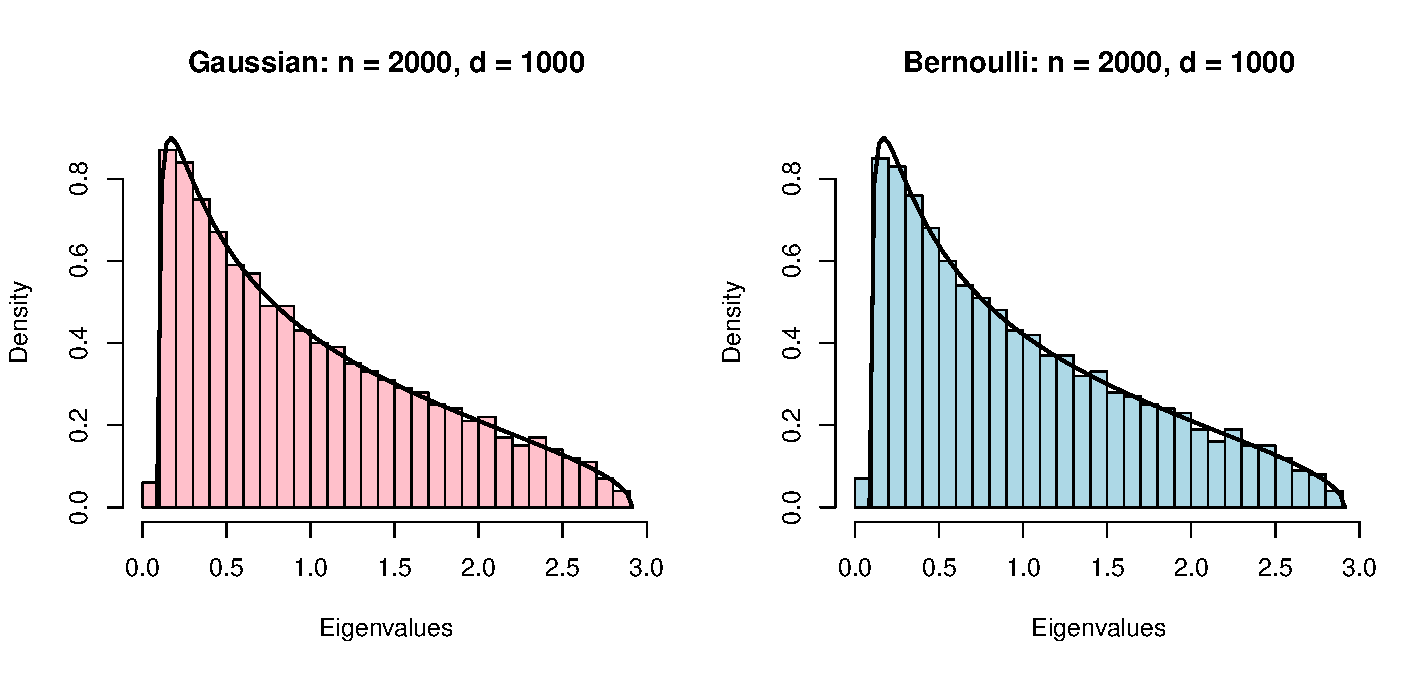
\includegraphics[width=\textwidth]{mp.pdf}
\caption{\it Empirical verification of the MP theorem when $n=2000$,
  $d=1000$. The left panel shows the empirical distribution of eigenvalues of
  $X^\T X/n$ when it has standard Gaussian entries, and the right panel shows 
  the same but when it has standardized Bernoulli entries. The black curve in
  each panel is the density of the MP law.}    
\label{fig:mp}
\end{figure}

Third, the Marchenko-Pastur theorem displays a remarkable phenomenon called
\emph{universality}: no matter the distribution of the elements of $Z$ that give
rise to our sample covariance matrix \smash{$\hSigma = X^\T X/n$} (recall the
relationship $X = Z \Sigma^{1/2}$), \emph{we get the same limit $F$} for the
spectral distribution of \smash{$\hSigma$}. This limit only depends on $\gamma$
and $H$. So for example, in the isotropic case, we learn that if we populate the
entries of $X$ with i.i.d.\ standardized (zero mean, unit variance) random
variables, whether they be Gaussian, Bernoulli, Poisson, t, etc., and plot a
histogram of the eigenvalues of $X^\T X/n$ for large $n$, then it is ``very
likely'' that they will look like they follow \eqref{eq:mp_law}. See again
Figure \ref{fig:mp}.  

Fourth, and last, it is worth emphasizing that the distribution $F$ from Theorem 
\ref{thm:mp} is the \emph{almost sure} limit of eigenvalues of \smash{$\hSigma =
  X^\T X/n$}. Interpreting this correctly can sometimes be challenging for
people learning this material for the first time. Let us be clear about what it
does \emph{not} say: the result does not imply that the eigenvalues of
\smash{$\hSigma$} for large $n$ will approximately concentrate around some
deterministic number. (This would be the case in classical asymptotics, with $n
\to \infty$ and $d$ fixed.) Rather, it means that the eigenvalues will exhibit a
\emph{predictable spread} for large $n$. In other words, when seeking to
empirically examine the statement in Theorem \ref{thm:mp}, as we did in Figure
\ref{fig:mp}, we do not need to average results over repetitions or anything
like that, because just a single draw of $X$ should produce eigenvalues that
approximately display the predicted spread. And if we simply redrew the Gaussian 
or Bernoulli entries, then we would (and should) get basically identical-looking
plots.   

\subsection{Deterministic equivalents}

It turns out that we can restate the Marchenko-Pastur theorem in modern (or at
least, not-so-classical) terms, using what is known as the language of
\emph{deterministic equivalents}. Two sequences of (deterministic or random)
matrices $A_n,B_n$, $n=1,2,3,\dots$ of growing dimension are said to be
asymptotically equivalent, written as $A_n \asymp B_n$, provided that for all
sequences $\Theta_n$, $n=1,2,3,\ldots$ that are bounded in trace
norm,\footnote{The trace norm of $\Theta \in \R^{n \times n}$ is
  \smash{$\|\Theta\|_* = \sum_{i=1}^n |\sigma_i(\Theta)|$}, where
  $\sigma_i(\Theta)$, $i=1,\dots,n$ are the singular value of
  $\Theta$. Equivalently, \smash{$\|\Theta\|_* = \tr[(\Theta^\T
    \Theta)^{1/2}]$}.}   
\[
\tr \big[ \Theta_n (A_n - B_n) \big] \to 0, \quad \text{as $n \to \infty$}. 
\]
This language gives us a way to cleanly state the MP theorem, as promoted by
\citet{dobriban2021distributed} (these authors also develop a ``calculus'' for
deterministic equivalents). The following is a transcription of a result by
\citet{rubio2011spectral}, that can be viewed as a generalized version of the
MP theorem.  

\begin{theorem}[\citealt{rubio2011spectral}]
\label{thm:rubio}
Let $X = Z \Sigma^{1/2} \in \R^{n \times d}$, where the entries of $Z$ are
i.i.d.\ from a distribution with zero mean, unit variance, and finite $8+\eta$ 
moment, for some $\eta>0$. Assume that as $n,d \to \infty$, the aspect ratio 
$\gamma_n = d/n$ remains bounded away from $0$ and $\infty$, as do the
eigenvalues of $\Sigma$. Then the resolvent of \smash{$\hSigma = X^\T X/n$} is
asymptotically equivalent to a deterministic matrix, namely:
\begin{equation}
\label{eq:rubio}
(\hSigma - zI)^{-1} \asymp (a_n \Sigma - zI)^{-1}, \quad \text{for $z \in \C  
  \setminus \R_+$},
\end{equation}
where $a_n$ is the unique solution of the fixed-point equation:
\begin{equation}
\label{eq:fixed_point}
\frac{1}{\gamma_n} \bigg( \frac{1}{a_n} - 1 \bigg) = \frac{1}{d} \tr \big[
\Sigma (a_n \Sigma - zI)^{-1} \big]. 
\end{equation}
\end{theorem}

We note that this theorem is quite general: it does not require $d/n$ to
actually converge to anything, nor require that the spectral distribution of
$\Sigma$ has a limit. Furthermore, asymptotic equivalence implies many
interesting things: for example, taking $\Theta_n = I/d$ in the definition
of asymptotic equivalence shows that \eqref{eq:rubio} implies convergence in 
Stieltjes transforms, which effectively recovers the original MP
result. However, there is much more we can learn from \eqref{eq:rubio},
including convergence of eigenvectors; see \citet{rubio2011spectral} for a
discussion.     

Lastly, as a particularly simple and hence notable consequence of Theorem
\ref{thm:rubio}, it is shown in \citet{dobriban2021distributed} that we can take
$z \to 0$ in \eqref{eq:rubio}, which gives
\begin{equation}
\label{eq:cov_deter_equiv}
\hSigma^{-1} \asymp \frac{1}{1 - \gamma_n} \Sigma^{-1},
\end{equation}
where we have used the fact (which can easily be verified) that $a_n =
1-\gamma_n$ solves the fixed-point equation \eqref{eq:fixed_point} in the case 
$z=0$. 

\section{Least squares analysis}

\def\Risk{\mathrm{Risk}}
\def\Bias{\mathrm{Bias}}

In this section, we will analyze the out-of-sample risk of least squares
regression in a proportional asympotics model, both as a warm-up for ridge
regression (the focus of the following sections), but also because it is an
certainly important result in its own right---as we alluded to in previous
lectures more than once. 

We consider the linear model
\begin{equation}
\label{eq:model}
Y = X\beta_0 + \epsilon,
\end{equation}
assuming as usual that $\epsilon \in \R^n$ has i.i.d.\ entries with mean zero
and variance $\sigma^2$, and $\epsilon \indep X$. To clearly lay out the
conditions on the features $X \in \R^{n \times d}$, we assume the following: 
\begin{itemize}
\item[(A1)] $X = Z \Sigma^{1/2}$, where the entries of $Z \in \R^{n \times d}$
  are i.i.d.\ with zero mean and unit variance;
\item[(A2)] the covariance matrix $\Sigma \in \R^{d \times d}$ has eigenvalues
  bounded away from $0$ and $\infty$;  
\item[(A3)] $d/n \to \gamma \in (0,1)$ as $n,d \to \infty$,
\end{itemize}
To emphasize, we are placing the restriction here that $\gamma < 1$, called the
\emph{underparametrized} regime. We will analyze the asymptotic risk of the
ordinary least squares estimator, which we can write as 
\begin{equation}
\label{eq:ls_rescaled}
\hbeta = (X^\T X/n)^{-1} X^\T Y/n.
\end{equation}
One can show that this is almost surely well-defined under the assumptions laid
out.\footnote{To be more precise, as $n,d \to \infty$ with $d/n \to \gamma \in
  (0,1)$, the minimum eigenvalue of $X^\T X/n$ will be almost surely lower
  bounded away from zero. This follows from what is called the Bai-Yin theorem 
  \citep{bai1993limit}, along with the fact that $\Sigma$ has eigenvalues
  bounded away from zero.}  
Now let $x_0 = \Sigma^{1/2} z_0$ be i.i.d.\ to the rows of $X$, and consider the
out-of-sample risk of least squares, conditional on $X$,
\begin{equation}
\label{eq:risk}
\Risk_X(\hbeta; \beta_0) = \E \big[ ( x_0^\T \hbeta - x_0^\T \beta_0 )^2
\,\big|\, X \big].
\end{equation}
By standard calculations, as covered previously, we can decompose the risk
\eqref{eq:risk} of the least squares estimator \eqref{eq:ls_rescaled} into bias
and variance terms; the bias term is zero, so the risk is pure variance,      
\begin{align}
\nonumber
\Risk_X(\hbeta; \beta_0) 
&= \frac{\sigma^2}{n} \tr\Big(\E [x_0 x_0^\T] \, (X^\T X/n)^{-1} \Big) \\
\nonumber
&= \frac{\sigma^2}{n}\tr\Big(\Sigma \big[ \Sigma^{1/2} (Z^\T Z/n) \Sigma^{1/2} 
  \big]^{-1} \Big) \\ 
\label{eq:ls_var}
&= \frac{\sigma^2 d}{n} \frac{1}{d} \tr \big[ (Z^\T Z/n)^{-1} \big].
\end{align}
There are now several ways to proceed to compute the limit of above line, all
based around the Marchenko-Pastur theorem. Of course, each way must arrive at
the same answer, which is
\begin{equation}
\label{eq:ls_risk_limit}
\Risk_X(\hbeta; \beta_0) \asto \sigma^2 \frac{\gamma}{1-\gamma},
\end{equation}
where to be clear, ``almost surely'' is to be interpreted with respect to the
distribution of $X$. Looking back at \eqref{eq:ls_var}, clearly $\sigma^2 d/n
\to \sigma^2 \gamma$, so in order to establish \eqref{eq:ls_risk_limit} it
suffices to prove that   
\begin{equation}
\label{eq:ls_var_limit}
\frac{1}{d} \tr \big[ (Z^\T Z/n)^{-1} \big] \asto \frac{1}{1-\gamma}.
\end{equation}
Below, we step through three routes for calculating this limit. But first, it is
worth emphasizing the behavior of the asymptotic risk profile in
\eqref{eq:ls_risk_limit}:  
\begin{quote}
\centering\it
The out-of-sample risk of least squares blows up as $\gamma \to 1$ from below,
that is, as we grow the aspect ratio until $d = n$ in the limit, least squares
regression exhibits catastrophic risk.  
\end{quote}
What happens past $\gamma = 1$? The answer may surprise you. We'll return to
this in the next lecture.  

\paragraph{Marchenko-Pastur theorem, followed by calculus.}  

We can recognize the left-hand side in \eqref{eq:ls_var_limit} in terms of the
Stieltjes transform of the spectral distribution $F_{Z^\T Z/n}$,  
\[
\frac{1}{d} \tr \big[ (Z^\T Z/n)^{-1} \big] = m_{F_{Z^\T Z/n}}(0).
\]
To study the limit of \smash{$m_{F_{Z^\T Z/n}}(0)$}, we can use the
Marchenko-Pastur theorem, transcribed in Theorem \ref{thm:mp}. This tells us
that $F_{Z^\T Z/n}$ converges weakly almost surely to $F$, the MP law in
\eqref{eq:mp_law}, hence we get convergence of Stieltjes transforms, so     
\[
m_{F_{Z^\T Z/n}}(0) \asto m_F(0).
\]
Fortunately, the Stieltjes transform of $F$ in \eqref{eq:mp_law} has an explicit
form, for real $z>0$:    
\begin{equation}
\label{eq:mp_stieltjes}
m(-z) = \frac{-(1 - \gamma + z) + \sqrt{(1 - \gamma + z)^2 + 4 \gamma z}}{2
  \gamma z}. 
\end{equation}
Since the limit as $z \to 0$ is indeterminate, we can use l'H{\^o}pital's rule
to calculate:   
\begin{align*}
\lim_{z \to 0} \, m(-z) 
&= \lim_{z \to 0} \, \frac{-1 + \frac{1+\gamma+z}
  {\sqrt{(1-\gamma+z)^2 + 4\gamma z}}}{2\gamma} \\
&= \frac{-1+\frac{1+\gamma}{1-\gamma}}{2\gamma} 
= \frac{1}{1-\gamma},
\end{align*}
which establishes the result in \eqref{eq:ls_var_limit}. 

\paragraph{Gaussian calculation, in expectation.} 

We can actually get away with a simpler calculation. Observe that the
Marchenko-Pastur theorem tells us that the limit of the left-hand side in
\eqref{eq:ls_var_limit} is both \emph{universal} and \emph{almost sure}, and
thus it suffices to compute it in the Gaussian case, in expectation. That is, it 
suffices to study the limit of
\[
\frac{1}{d} \tr \Big[ \E\big[ (Z^\T Z/n)^{-1} \big] \Big], \quad \text{for $Z$ 
  having i.i.d.\ $N(0,1)$ entries.}
\]
In this case, $Z^\T Z$ is Wishart, and $(Z^\T Z)^{-1}$ is inverse Wishart, so it
has a known expectation $\E[(Z^\T Z)^{-1}] = I/(n-d-1)$. This means that
\[
\frac{1}{d} \tr \Big[ \E\big[ (Z^\T Z/n)^{-1} \big] \Big] = \frac{n}{n-d-1} \to
\frac{1}{1-\gamma}, 
\]
as desired, which establishes \eqref{eq:ls_var_limit}.

\paragraph{Deterministic equivalents.}

The formulation of the Marchenko-Pastur theorem in terms of deterministic
equivalents, as transcribed in Theorem \ref{thm:rubio}, leads to the simplest
calculation. To be precise, in order to use this result, we must assume a bit
more about the distribution of entries of $Z$: recall that we must assume that
it has $8+\eta$ moments, for some $\eta>0$. Now recall that an implication of
this theorem is that we have the deterministic equivalence
\eqref{eq:cov_deter_equiv}, in the isotropic case. But we are in this
case---there are no appearances of $\Sigma$ in \eqref{eq:ls_risk_limit}.  A 
direct implication of \eqref{eq:cov_deter_equiv} (just use $\Theta_n = I/d$ in
the definition of asymptotic equivalence) is that   
\[
\frac{1}{d} \tr \big[ (Z^\T Z/n)^{-1} \big] \quad \text{and} \quad
\frac{1}{1-d/n} \frac{1}{d} \tr(I) = \frac{1}{1-d/n} \quad \text{have the same 
  asymptotic limit}, 
\]
and we can just read off that right-hand quantity converges to $1/(1-\gamma)$,
which again proves \eqref{eq:ls_var_limit}.   

\section{Ridge analysis}

On to the analysis of ridge regression, which we will break up into two cases:
the isotropic case, in which $\Sigma = I$, and the general case, in which
$\Sigma$ is arbitrary (subject to minor restrictions, as usual, like eigenvalues
bounded away from $0$ and $\infty$). In the isotropic case, we will be able to
analyze the ridge risk with the random matrix theory tools introduced
previously.  The general $\Sigma $ case will be more challenging, and there we 
will simplify the bias calculation by taking underlying signal $\beta_0$ to be
random, i.e., by imposing a prior on $\beta_0$. We will discuss briefly what
happens for general $\Sigma$ and fixed $\beta_0$ at the end.          

As in the least squares analysis, we will assume the linear model
\eqref{eq:model}, and will use similar assumptions to (A1)--(A3) for the feature   
model, but considering the full range $\gamma \in (0,\infty)$. To be specfic, we
assume:    
\begin{itemize}
\item[(B1)] $X = Z \Sigma^{1/2}$, where the entries of $Z \in \R^{n \times d}$
  are i.i.d.\ with zero mean, unit variance, and finite $8+\eta$ moment, for
  some $\eta>0$; 
\item[(B2)] the covariance matrix $\Sigma \in \R^{d \times d}$ has eigenvalues
  bounded away from $0$ and $\infty$, and satisfies \smash{$F_\Sigma \dto H$},
  as $n,d \to \infty$; 
\item[(B3)] $d/n \to \gamma \in (0,\infty)$ as $n,d \to \infty$.
\end{itemize}

We will analyze the asymptotic out-of-sample risk \eqref{eq:risk} of the ridge
estimator. (Recall that this is conditional on $X$.) For convenience we will
reparametrize the ridge estimator as    
\begin{equation}
\label{eq:ridge_rescaled}
\hbeta = (X^\T X/n + \lambda I)^{-1} X^\T Y/n,
\end{equation}
which can either be seen as the original ridge estimator in \eqref{eq:ridge_sol} 
with tuning parameter $n\lambda$, or as the solution in the original ridge
problem \eqref{eq:ridge} after rescaling the loss term by $1/n$.  

At the outset, we will record the following facts, which you'll verify on the
homework. The bias and variance components of the risk \eqref{eq:risk} of the
ridge estimator \eqref{eq:ridge_rescaled} are:     
\begin{align}
\label{eq:ridge_bias}
\Bias_X(\hbeta; \beta_0) &= \lambda^2 \beta_0^\T (\hSigma + \lambda I)^{-1}
  \Sigma (\hSigma + \lambda I)^{-1} \beta_0 \\ 
\label{eq:ridge_var}
\Var_X(\hbeta) &= \frac{\sigma^2}{n} \tr \big[ \hSigma ( \hSigma + \lambda
  I)^{-2} \Sigma \big],
\end{align}
respectively, where recall \smash{$\hSigma = X^\T X/n$}. It is worth noting that
the variance does not depend on $\beta_0$. 

\subsection{Isotropic $\Sigma$, fixed $\beta_0$}

We consider the isotropic case, $\Sigma = I$. We will assume that $\|\beta_0\|_2
= r$ (which is a constant that does not vary with $n,d$), for the true signal
vector in \eqref{eq:model}. Below we analyze the bias and variance separately. 

\paragraph{Bias analysis.}

When $\Sigma = I$, the bias \eqref{eq:ridge_bias} becomes 
\begin{equation}
\label{eq:ridge_bias_iso}
\Bias_X(\hbeta; \beta_0) = \lambda^2 \beta_0^\T (\hSigma + \lambda I)^{-2}
\beta_0.  
\end{equation}
The key is to recognize this as the derivative with respect to $\lambda$ of a
certain functional,
\begin{equation}
\label{eq:deriv_trick_iso}
\beta_0^\T (\hSigma + \lambda I)^{-2} \beta_0 = - \frac{d}{d\lambda} \Big \{
\beta_0^\T (\hSigma + \lambda I)^{-1} \beta_0 \Big\}.
\end{equation}
By the deterministic equivalence in \eqref{eq:rubio} from Theorem
\ref{thm:rubio}, we know (just take $\Theta_n = \beta_0\beta_0^\T$ in the 
definition of deterministic equivalence) that   
\[
\beta_0^\T (\hSigma + \lambda I)^{-1} \beta_0 \quad \text{and} \quad 
\beta_0^\T (a_n I + \lambda I)^{-1} \beta_0 = \frac{r^2}{a_n + \lambda} \quad
\text{have the same asymptotic limit}. 
\]
We need to figure out the asymptotic limit of $a_n$. Instead of trying to
solve the fixed-point equation \eqref{eq:fixed_point}, it is easier to ``sneak
up on the answer'', by approaching it this way:
\[
\frac{1}{d} \tr \big[ (\hSigma + \lambda I)^{-1} \big] \quad \text{and} \quad 
\frac{1}{d} \tr \big[ (a_n I + \lambda I)^{-1} \big] = \frac{1}{a_n + \lambda}
\quad \text{have the same asymptotic limit},  
\]
and by the standard MP asymptotics, we know that the left-hand side converges
almost surely to $m_F(-\lambda)$, the Stieltjes transform
\eqref{eq:mp_stieltjes} of the MP law \eqref{eq:mp_law}, evaluated at
$-\lambda$. Thus we have $1/(a_n + \lambda) \to m_F(-\lambda)$, and 
\[
\beta_0^\T (\hSigma + \lambda I)^{-1} \beta_0 \asto r^2 m_F(-\lambda).
\]
Returning to \eqref{eq:deriv_trick_iso}, some calculations involing Vitali's
theorem (whose details we omit) show that we may exchange the order of the 
derivative and the limit, yielding 
\[
\beta_0^\T (\hSigma + \lambda I)^{-2} \beta_0 \asto r^2 m'_F(-\lambda), 
\]
and finally from \eqref{eq:ridge_bias_iso}, 
\begin{equation}
\label{eq:ridge_bias_iso_limit}
\Bias_X(\hbeta; \beta_0) \asto \lambda^2 r^2 m'_F(-\lambda).
\end{equation}

\paragraph{Variance analysis.}

When $\Sigma = I$, the variance \eqref{eq:ridge_var} becomes 
\begin{align*}
\Var_X(\hbeta)
&= \frac{\sigma^2}{n} \tr \big[ \hSigma ( \hSigma + \lambda I)^{-2} \big] \\ 
&=\frac{\sigma^2}{n} \Big( \tr \big[ ( \hSigma + \lambda I)^{-1} \big] - 
\lambda \, \tr \big[ (\hSigma + \lambda I)^{-2} \big] \Big),
\end{align*}
where in the second line we added and subtracted $\lambda I$ to the leading
$\hSigma$ inside the trace. Calculation of the limit of the above is now
straightforward, given what we have done above for the bias. After multiplying 
and dividing by $d$, this is the same as 
\[
\frac{\sigma^2 d}{n} \bigg( \frac{1}{d} \tr \big[ ( \hSigma + \lambda I)^{-1} 
\big] - \frac{\lambda}{d} \tr \big[ (\hSigma + \lambda I)^{-2} \big] \bigg).  
\]
The first term inside the parentheses has limit $m_F(-\lambda)$ by standard MP
asymptotics, and the second term has limit $-\lambda m'_F(-\lambda)$ by the same
arguments as above. Thus   
\begin{equation}
\label{eq:ridge_var_iso_limit}
\Var_X(\hbeta) \asto \sigma^2 \gamma \big( m_F(-\lambda) - \lambda 
m'_F(-\lambda) \big).
\end{equation}

\paragraph{Putting it together.}

Adding the bias \eqref{eq:ridge_bias_iso_limit} and variance results
\eqref{eq:ridge_var_iso_limit} together, we get
\begin{equation}
\label{eq:ridge_risk_iso_limit}
\Risk_X(\hbeta; \beta_0) \asto \sigma^2 \gamma 
\Big( m_F(-\lambda) - \lambda (1 - \alpha \lambda) m'_F(-\lambda) \Big), 
\end{equation}
where we have introduced $\alpha = r^2 / (\sigma^2 \gamma)$. Note that we can
think of this as $\alpha = \mathrm{SNR} / \gamma$, where $\mathrm{SNR} = r^2 /
\sigma^2$ can be thought of the signal-to-noise ratio for our problem. Recall
that $m_F$ is the Stieltjes transform \eqref{eq:mp_stieltjes} of the MP law
\eqref{eq:mp_law}. 

It can be shown that the asymptotically optimal tuning parameter value---the one
minimizing the asymptotic risk in \eqref{eq:ridge_risk_iso_limit}, is $\lambda^*
= 1/\alpha$. This has the general behavior that we would intuitively expect: it
shrinks (less regularization) as $\alpha$ grows (higher SNR), or equivalently,
it grows (more regularization) as $\alpha$ shrinks (lower SNR). Moreover, the
asymptotic risk \eqref{eq:ridge_risk_iso_limit} at the tuning parameter value
$\lambda^* = 1/\alpha$ simplifies to      
\[
\sigma^2 \gamma m_F(-1/\alpha) = \sigma^2 \frac{-(1 - \gamma + 1/\alpha) + 
  \sqrt{(1 - \gamma + 1/\alpha)^2 + 4\gamma / \alpha}}{2\gamma /\alpha}.     
\]
It is worth emphasizing that this \emph{does not blow up at $\gamma = 1$}, 
unlike the asymptotic least squares risk \eqref{eq:ls_risk_limit}. 
Regularization has saved the day! 

\subsection{General $\Sigma$, random $\beta_0$}

We consider the general $\Sigma$ case. We follow the general approach in
\citet{dobriban2018high}, but adopt the perspective of deterministic equivalents
as suggested by \citet{dobriban2021distributed}. We will place a spherical prior on $\beta_0$,
such that       
\begin{equation}
\label{eq:prior}
\E[\beta_0 \beta_0^\T] = \frac{r^2}{d} I.
\end{equation}
Note this implies $\E \|\beta_0\|_2^2 = r^2$. Our measure of risk is now a kind
of \emph{Bayes} out-of-sample prediction risk,  
\begin{equation}
\label{eq:ridge_risk_bayes}
\Risk_X(\hbeta) = \E \big[ ( x_0^\T \hbeta - x_0^\T \beta_0 )^2 \,\big|\,
X \big],
\end{equation}
where to be clear the expectation is over $\epsilon, x_0$, and $\beta_0$ (all
independent), and conditional on $X$. 

\paragraph{Bias analysis.}

For the bias, after taking an expectation in \eqref{eq:ridge_bias} over
$\beta_0$ drawn from \eqref{eq:prior}, we get
\begin{align}
\nonumber
\Bias_X(\hbeta) 
&= \lambda^2 \E \Big[ \beta_0^\T (\hSigma + \lambda I)^{-1} \Sigma (\hSigma + 
  \lambda I)^{-1} \beta_0 \Big] \\
\label{eq:ridge_bias_bayes}
&= \frac{\lambda^2 r^2}{d} \tr \big[ \Sigma (\hSigma + \lambda I)^{-2} \big],
\end{align}
where in the second line we used trace rotation, as in $\beta_0^\T M \beta_0 = 
\tr(\beta_0 \beta_0^\T M)$ for a matrix $M$, and invoked the prior
\eqref{eq:prior}. To compute the limit of \eqref{eq:ridge_bias_bayes}, the key,
similar to the isotropic case, is to recognize that   
\begin{equation}
\label{eq:deriv_trick_bayes}
\frac{1}{d} \tr \big[ \Sigma (\hSigma + \lambda I)^{-2} \big] = -
\frac{d}{d\lambda} \bigg \{ \frac{1}{d} \tr \big[ \Sigma (\hSigma + \lambda  
I)^{-1} \big] \bigg\}.   
\end{equation}
By the deterministic equivalence in \eqref{eq:rubio} from Theorem
\ref{thm:rubio}, we know that
\[
\frac{1}{d} \tr \big[ \Sigma (\hSigma + \lambda I)^{-1} \big] \quad \text{and}
\quad \frac{1}{d} \tr \big[\Sigma (a_n \Sigma + \lambda I)^{-1} \big] \quad
\text{have the same asymptotic limit}.
\]
Again, we need to figure out the asymptotic limit of $a_n$. Solving the
fixed-point equation \eqref{eq:fixed_point} will not be possible, but
nonetheless we can ``sneak up on the answer'', by rewriting
\eqref{eq:fixed_point} for $z = -\lambda$ as
\[
\frac{1}{a_n}  = 1 + \frac{\gamma_n}{d} \tr \big[ \Sigma (a_n \Sigma + \lambda 
I)^{-1} \big]. 
\]
What does this remind you of? Recall the Silverstein equation
\eqref{eq:silverstein}; at $z = -\lambda$, this can be rewritten as     
\[
\frac{1}{\lambda v_F(-\lambda)} = 1 + \gamma \int \frac{s}{s \lambda
  v_F(-\lambda) + \lambda} \, dH(s). 
\]
Writing $a$ for the limit of $a_n$, note that the second-to-last display
converges as $n,d \to \infty$ to the last display, with the relationship $a =
\lambda v_F(-\lambda)$. That is, to be clear, we have learned that $a_n \to
\lambda v_F(-\lambda)$, where $v_F$ is the companion Stieltjes transform of the
limiting spectral distribution $F$ from the MP theorem, and 
\[
\frac{1}{d} \tr \big[ \Sigma (a_n \Sigma + \lambda I)^{-1} \big] =
\frac{1}{\gamma_n} \bigg( \frac{1}{a_n} - 1 \bigg) \to \frac{1}{\gamma} 
\bigg( \frac{1}{\lambda v_F(-\lambda)} - 1 \bigg),
\]
and therefore 
\[
\frac{1}{d} \tr \big[ \Sigma (\hSigma + \lambda I)^{-1} \big] \asto
\underbrace{\frac{1}{\gamma} \bigg( \frac{1}{\lambda v_F(-\lambda)} - 1   
  \bigg)}_{\phi_F(-\lambda)}. 
\]
Returning to \eqref{eq:deriv_trick_bayes}, after checking some conditions (whose 
details we omit), we may exchange the order of the derivative and the limit,
yielding  
\[
\frac{1}{d} \tr \big[ \Sigma (\hSigma + \lambda I)^{-2} \big] =
\phi'_F(-\lambda),
\]
and finally from \eqref{eq:ridge_bias_bayes}, 
\begin{equation}
\label{eq:ridge_bias_bayes_limit}
\Bias_X(\hbeta) \asto \lambda^2 r^2 \phi'_F(-\lambda). 
\end{equation}

\paragraph{Variance analysis.}

For the variance \eqref{eq:ridge_var}, by adding and subtracting $\lambda I$ in
the leading \smash{$\hSigma$} in the trace, we get 
\begin{align*}
\Var_X(\hbeta) 
&= \frac{\sigma^2 d}{n} \Big( \tr \big[ \Sigma ( \hSigma + \lambda I)^{-1} \big] -
  \lambda \, \tr \big[ \Sigma (\hSigma + \lambda I)^{-2} \big] \Big) \\
&= \frac{\sigma^2 d}{n} \bigg( \frac{1}{d} \tr \big[ \Sigma ( \hSigma + \lambda 
  I)^{-1} \big] -\frac{\lambda}{d} \tr \big[ \Sigma (\hSigma + \lambda I)^{-2} 
  \big] \bigg).
\end{align*}
We can apply the same logic as developed for the bias to each of the two terms
above inside the parentheses: the first has limit $\phi_F(-\lambda)$ and the
second has limit $-\lambda \phi'_F(-\lambda)$, therefore   
\begin{equation}
\label{eq:ridge_var_limit}
\Var_X(\hbeta) \asto \sigma^2 \gamma \big( \phi_F(-\lambda) - \lambda 
\phi'_F(-\lambda) \big).
\end{equation}
We remark that this variance calculation did not require the prior assumption
\eqref{eq:prior}.  

\paragraph{Putting it together.}

Adding the bias \eqref{eq:ridge_bias_bayes_limit} and variance results
\eqref{eq:ridge_var_limit} together, we get
\begin{equation}
\label{eq:ridge_risk_bayes_limit}
\Risk_X(\hbeta) \asto \sigma^2 \gamma \Big( \phi_F(-\lambda) - \lambda (1 -
\alpha \lambda) \phi'_F(-\lambda) \Big),  
\end{equation}
where as before $\alpha = r^2 / (\sigma^2 \gamma)$. Recall that 
 \[
\phi_F(z) = -\frac{1}{\gamma} \bigg( \frac{1}{z v_F(z)} + 1 \bigg),
\]
and $v_F$ is the companion Stieltjes transform of the limit $F$ of the spectral
distribution of \smash{$\hSigma$}, as given by Theorem \ref{thm:mp}.

It is worth noting the close similarity between the results in the general
$\Sigma$ case \eqref{eq:ridge_risk_bayes_limit} and in the $\Sigma = I$ case  
\eqref{eq:ridge_risk_iso_limit}, where $\phi_F$ in the latter plays the role of
$m_F$ in the former. In the general $\Sigma$ case, while we were able to obtain
an exact expression \eqref{eq:ridge_risk_bayes_limit} for the limiting risk,
this expression is no longer explicit, as the solution $v_F$ to the
Silverstein equation \eqref{eq:silverstein} is not explicit for general $H$. 

Still, remarkably, it is shown in \citet{dobriban2018high} that the
asymptotically optimal tuning parameter value---the one that minimizes the 
asymptotic risk in \eqref{eq:ridge_risk_bayes_limit}, is once again $\lambda^*   
= 1/\alpha$, regardless of the sequence of covariance matrices $\Sigma$
(regardless of $H$). Their argument is too clever to pass by in these notes, and
so we outline it here. Specialize to the case where $\epsilon \sim N(0,\sigma^2
I)$ and $\beta_0 \sim N(0, (r^2/d) I)$ in \eqref{eq:model} and \eqref{eq:prior},
respectively. As we argued previously (recall \eqref{eq:normal_bayes},
\eqref{eq:ridge_bayes}), note that the ridge estimator with
\[
\lambda^*_n = (\sigma^2 d)/(r^2 n)
\]
is the Bayes estimator in this normal-normal model. In fact, it is the unique
Bayes estimator, and thus it obtains a smaller Bayes risk than any other
estimator. Note that $\lambda^*_n \to \sigma^2 \gamma / r^2= \lambda^*$. Since 
the limit of the risk in \eqref{eq:ridge_risk_bayes} is both universal and
almost sure, we can use the optimality of $\lambda^*_n$ as argued above, along
with an equicontinuity argument, to show that $\lambda^* = 1/\alpha$ is optimal
in the limit.  

\subsection{General $\Sigma$, fixed $\beta_0$?}

For a general $\Sigma$, the behavior of ridge regression along an arbitrary
sequence of fixed signal vectors $\beta_0$ can actually be surprisingly
exotic. First, it is no longer true that the optimal limiting tuning parameter
value $\lambda^*$ is simply $1/\alpha$, and furthermore, it is no longer true
that it is even positive (it may be zero). The reason for this exotic behavior
is the bias term \eqref{eq:ridge_bias}, specifically the way that it depends on
the joint geometry of $\beta_0$ and $\Sigma$.

The results describing the asymptotic risk here are very recent, and relate to
the study of overparametrization, so we will touch on them in the next lecture. 

\bibliographystyle{plainnat}
\bibliography{../../common/ryantibs}

\end{document}
